\documentclass[10pt,a4paper]{article}
\usepackage[utf8]{inputenc}
\usepackage[french]{babel}
\usepackage[T1]{fontenc}
\usepackage{amsmath}
\usepackage{amsfonts}
\usepackage{amssymb}
\usepackage{graphicx}
\usepackage{hyperref}
\usepackage[left=2cm,right=2cm,top=2cm,bottom=2cm]{geometry}
\usepackage{siunitx}
\usepackage{multicol}
\author{Baptiste Rouger}
\title{Lab Notebook MSC}

\setcounter{secnumdepth}{0}

\begin{document}
\maketitle

\tableofcontents

\newpage

\section{15 Jan 2018}

\begin{itemize}
    \item Début d'installation sur le PC
    \item Cassage de ArchLinux
    \item Rangement de la salle de manip et mise en place de la salle de manip
    \begin{itemize}
        \item Raccourcissement des plus longues barres de la cage qui gênaient.
        \item Réorganisation de la salle
    \end{itemize}
    \item Lecture de la review de Mathieu
\end{itemize}
\noindent Comment la température ambiante influence la fermeture des feuilles? \\
Comment la fermeture des feuilles affecte la température de celles-ci?

\section{16 Jan 2018}
\begin{itemize}
    \item Installation de Debian sur le PC
    \item Installation des logiciels importants sur le PC
    \item Mise en place de la première manip test pour la \textbf{nutation}: début à \textbf{15h52}, fin à \textbf{10h42} le 17 Jan 2018. Les données sont situées sur Alfred: /mnt/data/manip/Baptiste/test\_16-01-2018.J'ai utilisé la plante "Abby" pour réaliser cette manip. Photo toutes les 90 secondes.
\end{itemize}

\section{17 Jan 2018}
\begin{itemize}
    \item Arrêt de la manip \textbf{test\_16-01-2018} à \textbf{10h42}
    \item Arrosage des plantes
    \item Récupération des données de la manip
    \item Création du film à partir des données de la manip (\textit{cf}\textsc{Protocole}~\ref{film})
    \item Réalisation du script \textbf{analysisScript.py} qui, à partir de photos stockées dans un dossier, réalise la timeline d'une ligne de pixel et la converti en image binaire
\end{itemize}

Le lien pour la vidéo: \url{http://uptobox.com/5x80eimcd7xu}\\

Le résultat du script \textbf{analysisScript.py} :\\

\includegraphics[width = \linewidth]{imTLBWv1.jpg}

\section{18 Jan 2018}
\begin{itemize}
    \item Début d'une deuxième manip pour observer la nutation (sur un plus long terme). Début à environ 12h30 \textbf{(heure pc décalée????)}. Il fait \SI{24.2}{\celsius} dans la pièce, 49\% d'humidité. On utilise la plante "Béa". Les numéro de protocole sont:
    \begin{itemize}
        \item arduino: 21608
        \item photos: 21821
    \end{itemize}
    \item Création du script appelé \textbf{anSc3.py} qui utilise la librairie skimage pour analyser les images et réaliser le graphe de mouvement.

\end{itemize}

\section{19 Jan 2018}
Je me suis penché sur le problème du maintien de la température et de l'humidité de la salle de manip avec Arduino (ainsi que la photopériode). J'ai pris en compte la mesure de ces données. Schéma :\\
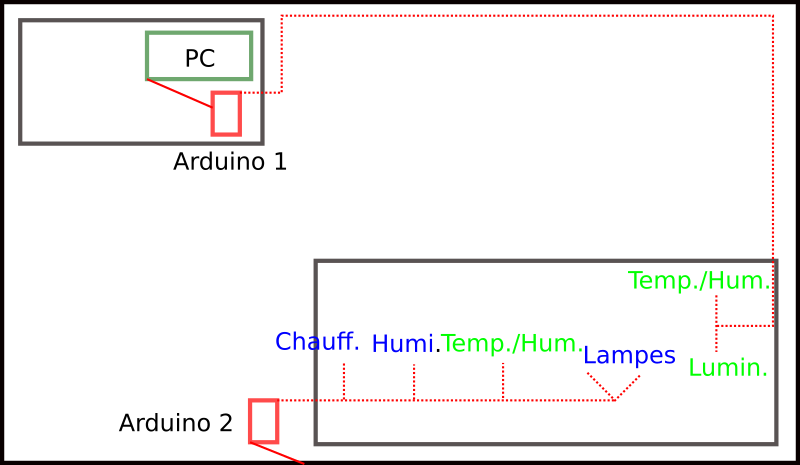
\includegraphics[width=0.6\linewidth]{schema_Arduino.png}

\section{20 Jan 2018}
J'ai refait le focus sur la jeune feuille, il n'était évidemment plus bon au bout de ces 2 jours et demi. $\Rightarrow$ Il serait intéressant de voir si l'auto focus pourrait compenser intelligemment cela.\\

Pour les scripts, je vais essayer de trouver la position du centre de la tige en utilisant une moyenne pondérée par le nombre de pixels consécutifs\\

J'ai modifié les scripts : je les ai séparé en deux : \texttt{TL.py} sert à créer l'image de la timeline, \texttt{Trajec.py} sert à récupérer la position moyenne de la tige. On peut entre les deux scripts retailler l'image.

\section{29 Jan 2018}
J'ai travaillé sur les scripts d'analyse de l'image, de récupération de la trajectoire et d'analyse en ondelette de ces trajectoires. J'ai découpé chaque étape et je les ai mises dans des scripts précédents qui prennent différents arguments (\textit{cf} \textsc{Protocole}~\ref{anaNut}).

J'ai fini le robot arduino qui contrôle la température, l'humidité et les lampes. Je le teste pour la nuit.

\section{30 Jan 2018}

Il y avait un problème dans le robot de contôle. J'ai dû modifier le code d'une part (problème de LOW et HIGH en output pour les relais). De plus, j'ai dû installer la librairie Time sur le pc de la salle de manip. J'ai vérifié que cela fonctionnait bien quelques minutes. Le nouveau code arduino pour le robot est joint dans le dépôt : \texttt{arduino\_Stat.ino}.\\

J'ai remarqué que la lampe numéro 2 (au dessus de la cage) ne fonctionne plus.

\section{31 Jan 2018}
Le robot de contrôle était encore bugé. Il se trouve que les relais se bloquent parfois et restent en position de contact alors qu'ils devraient couper le courant. Cela n'arrive que quand on branche la grosse lampe. Peut-être tire-t-elle trop de courant pour notre carte de relais. Il faudra voir si la carte est théoriquement capable de supporter les intensités que nous lui faisons traverser.\\

J'ai également retravaillé les codes d'analyse d'images. Ils sont toujours découpés en trois parties, mais maintenant on peut spécifier plusieurs lignes à \texttt{1-TL.py} pour éviter d'avoir à relancer le process des images trop de fois. Par ailleurs, j'utilise maintenant numpy.savetxt pour sauver la trajectoire en csv dans \texttt{2-Traj.py}, ainsi que numpy.loadtxt pour la charger dans \texttt{3-WL.py}. J'ai aussi nettoyé le code de tous les commentaires de débugage inutiles.

\section{01 Fev 2018}
Le robot de contrôle semble avoir grillé la lampe d'aurore ! De plus, il semble qu'avec le temps l'horloge de l'arduino se décale. Je vais essayer de voir de combien en combien de temps. Pour cela, j'ai pris un screen avec l'heure de l'arduino et l'heure du PC. Celui-ci se situe dans le dossier Pictures de manip.\\
On a réparé le robot, il fonctionne actuellement avec uniquement la lampe de jour et le chauffage. On a branché à la fois l'arduino et la plaque de relais avec des transfos, plus lien usb.\\

J'ai lancé une manip avec deux plantes : Béa et Clara. Début à 17h58. Il fait \SI{24}{\celsius}, la température est régulée par le robot. On a pas encore refait l'arduino chagé de capter la température, l'humidité et la luminosité, donc ces donénes ne seront pas présentes.

\section{02 Fev 2018}
J'ai refermé le robot de contrôle qui doit marcher normalement. J'ai changé le code arduino pour que le chauffage fonctionne aussi quand minute\%5 = 1 car la température descendait.\\

J'ai aussi commencé à faire le robot de mesure de la température, humidité et luminosité. Pour l'instant il n'y a que la luminosité qui fonctionne, avec un code pris dans les exemples d'adafruit. Il me faut une résistance pour monter le capteur de température et d'humidité.


\section{05 Fev 2018}
Le robot a planté pendant la nuit, la tepérature ce matin dans la salle était de \SI{312}{\celsius}. De plus, on a une grosse chute de l'humidité (environ 30\%).\\

La manip de Clara a bougé hors du cadre le 04 à partir de la photo 9h48. Je l'ai donc arrêtée ce matin vers 11h. J'ai lancé la conversion en film (elle ne semble pas avoir beaucoup bougé), ainsi que l'analyse d'image.\\

J'ai refait le focus pour la manip avec Béa.\\

Il me semble que l'on ne pourra pas utiliser plus d'un capteur de luminosité avec Arduino car celui ci se fixe dans des pins spéciaux (vers les 6 mâles groupés).\\

On a aussi intallé le relai statique pour alimenter le nouveau chauffage, pour voir si ceux là fonctionnent mieux que les relais mécaniques.

\section{06 Fev 2018}
La température était trop faible dans la pièce ce matin. Il semble qu'il faille mettre le chauffage à fond car sinon il ne fonctionne pas tout le temps (à 4 il est souvent éteint alors qu'il est sensé être allumé). De plus, comme j'avais peut que cela ne régule pas bien, j'ai également remis le chauffage 2 minutes toutes les 5 minutes (2' chauffe, 3' repos) avec arrêt si la température est supérieure à \SI{24}{\celsius}.\\

J'ai rempoté toutes les petites caramboles (18) dans de plus grands pots. J'ai mis au fond des pots une épaisseur de tissu pour éviter que la terre de bruyère ne s'en aille. Puis une couche de billes d'argile. Ensuite un mélange de billes d'argile et de terre de bruyère (environ un volume de billes pour 5-6 volumes de terre). Enfin, une couche de terre de bruyère seule. J'ai ajouté à chaque fois un peu de la terre du pot d'origine près des racines.\\ J'ai arrosé et complété la terre qui manquait. J'ai laissé un peu de terre de bruyère dans un pot dans la sale au cas où on ait besoin de compléter les pots à nouveau.\\
Les nouvelles plantes s'appellent :

\begin{multicols}{4}
    \begin{enumerate}
        \item Athéna
        \item Borée
        \item Chloris
        \item Déméter
        \item Éos
        \item Fortuna
        \item Gaia
        \item Hygie
        \item Io
        \item Jupiter
        \item Khnoum
        \item Léto
        \item Maïa
        \item Nyx
        \item Ouranos
        \item Pan
        \item Qébahout
        \item Rê
    \end{enumerate}
\end{multicols}

\section{12 Fev 2018}
J'ai oublié d'inscrire que le 08 Fev 2018, j'ai lancé une manip avec deux plantes : Béa et Clara. Je crois qu'elles ont beaucoup bougé pendant la prise de photos. L'expé est toujours en train de tourner.\\

J'ai cherché comment faire fonctionner nos 2 capteurs de luminosité en même temps sur le même arduino. Il semble donc qu'on puisse relier les broches SCL des deux capteurs ensemble avec une résistance, de même pour SDA. J'ai trouvé cette info sur \url{http://www.learningaboutelectronics.com/Articles/Multiple-I2C-devices-to-an-arduino-microcontroller.php}


\section{15 Fev 2018}
Lancement d'une manip avec deux plantes : Diana et Jupiter. Je l'ai lancée à 12h11.\\

Il y a eu beaucoup de changements dnas les scripts d'analyse des images. Maintenant, pour créer la timeline, il faut cliquer dans les images à la hauteur de la ligne que l'on veut prendre. L'intervalle entre 2 "picking" est une des entrées du script.  De plus, le script prend en entrée deux indices pour crop l'image de manière à réduire la taille du total et avoir une distinction de la tige plus nette. \textit{cf} \textsc{Protocole}~\ref{anaNut} pour plus de détails sur l'utilisation.\\ J'ai aussi enlevé le deuxième script \texttt{2-Traj.py} car ceci est fait dans le premier à présent.

\section{19 Fev 2018}
Arrêt de la manip avec Diana et Jupiter. Récupération et traitement des données.\\
Ajout de la sauvegarde des photos avec ligne rouge sélectionnée dasn \texttt{1-TL.py}.\\
Finition de l'Arduino sensor et installation dasn la serre. Le script python de récupération des données fonctionne. Il est situé dans \texttt{/mnt/data/manips/Baptiste/ArdSense}

\section{20 Fev 2018}
J'ai fini de mettre en place l'Arduino Sensor qui enregistre maintenant la température, l'humidité et la luminosité. J'ai disposé les capteurs sur une petite plaque de carton, principalement pour maintenir le capteur de luminosité à plat. J'ai disposé ce carton sur une des deux potences pour que la mesure de la luminosité soit proche de celle reçue par la plante.\\
J'ai dû redémmarer l'ordinateur parce qu'un appareil photo n'était pas détecté par le pc. En faisant cela, l'heure de l'ordi a changé...\\

Début de la manip avec Béa et Carla à 12h40. Je teste cette fois de tenir les autres feuilles en les entourant de fil. Je teste aussi le nouveau support de fond noir.\\

Changement de manip : j'ai relancé une manip (toujours avec Béa et Clara), cependant j'ai éloigné les plantes de l'appareil photo. Ainsi, le focus est bon, ainsi que le niveau de zoom. Le début est à 14h56. L'échellle est présente sur deux photos autour de 16h46.

\section{28 Fev 2018}
J'ai travaillé sur un modèle qui décrit le mouvement de nutation de la tige comme un ressort. Le code du modèle peut-être trouvé ici : \url{https://github.com/rougerbaptiste/elaStem}.

J'ai lancé une manip (toujours les mêmes conditions : \SI{24}{\celsius}, 12h de photopériode) avec Béa et Elisabeth à 15h42.


\section{02 Mar 2018}
J'ai refait la mise au point des appareils photos sur les manips.\\

J'ai rempoté la plus grande des plantes dans un pot plus grand. De plus, je l'ai taillée pour qu'elle est une taille plus facile à travailler, et je teste de faire une bouture avec ce que j'ai enlevé de la taille car le bout avait l'air bien vivace.\\
J'ai aussi remis un peu de terre dans les pots qui en manquaient.\\
J'ai repéré plusieurs caramboles qui sont dans des petits pots et qu'il faudra rempoter prochainement.

\section{06 Mar 2018}
J'ai rempoté deux plantes qui en avaient besoin (une petit pot, une presque plus de terre). Je vérifierai si d'autres doivent être rempotées.\\
Il fait presque \SI{25}{\celsius} dans la pièce ce matin parce que le temps s'est réchauffé et que le radiateur supplémentaire chauffait trop.\\

J'ai arrêté la manip sur [009,002] parce que la nutation était finie. J'ai remarqué que sur cette manip, certaines photos sont très sombres indépendament des periodes de jour/nuit. C'est sur cette manip que je testais le nouveau fond bleu.

\section{12 Mar 2018}
Les manips ont été arrêtées jeudi dernier. J'essaie de faire descendre la température de la pièce à \SI{20}{\celsius} sans grand succès (\SI{22}{\celsius} environ actuellement) pour lancer une nouvelle série de manips à cette température. \\
La première expé utilisera deux plantes : Béa et Fleur.\\
J'attends avant de lancer la manip car le robot de contrôle de la température et de la lumière ne fonctionne plus. Je l'ai modifié pour qu'il contrôle les trois lampes :
\begin{description}
    \item [\SI{2700}{\kelvin}] lampe d'aube : de 8h à 20h
    \item [\SI{6000}{\kelvin} \#1] lampe de jour : de 9h à 19h
    \item [\SI{6000}{\kelvin} \#2] lampe de zénith : de 11h à 13h
\end{description}

\section{14 Mar 2018}
Le robot doit (enfin!) marcher, maintenant chacun des câbles est lié à 2 relais : un statique qui ne craint pas le retour de courant des lampes et des charges inductives, et un mécanique qui coupe correctement le courant. Je dois aller voir Arnaud cet après-midi pour mettre tout cela en boîte.\\

Hier, j'ai lancé une manip avec Béa et Fleur à 18h10 hier soir. J'ai constaté ce matin que le flash externe semble parfois avoir des problèmes de régulation : certaines photos sont complètement noires.

\section{15 Mar 2018}
Je laisse tourner la manip en cours car Béa nute bien. L'autre plante a malheureusement un defaut avec e flash qu'il faudra régler (à voir dans les configurations de l'appareil photo). Je vais interrompre la manip ce soir car je ne pourrait pas être là demain.\\

À l'heure actuelle, ArdStat n'est pas prêt (et pas sûr qu'il le soit aujourd'hui car je pense qu'on aura pas le boîtier.)\\

J'ai refait les analyses des manips précédentes. J'ai fait un changement dasn le code : les axes des graphes finaux sont définis manuellement pour enlever les valeurs extrèmes abérantes et ainsi voir l'allure de la courbe.


\newpage
\begin{center}
    {\Huge Protocoles}
\end{center}
\appendix
\setcounter{secnumdepth}{1}

\section{Creation du film à partir des images\label{film}}
On utilise la commande \texttt{mencoder "mf://*.jpg" -mf w=320:h=240:fps=12:type=jpeg -ovc lavc -o output.avi}


\section{Analyse des images de la nutation\label{anaNut}}
\begin{enumerate}
    \item On a mis toutes les photos du film dans un dossier. On récupère le chemin d'accès à ce dossier.
    \item On utilise la commande : \texttt{python 1-TL.py Path ReadEvery WindowScale XStart XStop SpacePic} avec \texttt{Path} est la localisation du dossier, \texttt{ReadEvery} est l'intervalle auquel on veut cliquer sur les photos pour sélectionner la ligne, \texttt{WindowScale} est un coefficient pour diminuer la taille de l'image affichée, \texttt{XStart} est le pixel à partir duquel on veut crop l'image, \texttt{XStop} est le pixel jusqu'auquel on veut crop l'image, et \texttt{SpacePic} est l'intervalle de temps entre les images.
    \item Enfin \texttt{python 2-WL.py Path CSV Scale} avec \texttt{Path} la localisation du dossier, \texttt{CSV} le nom du fichier csv créé par \texttt{2-Trajec.py} et \texttt{Scale} la taille d'un pixel en cm.
\end{enumerate}




\end{document}
